\begin{notechapter}
\chapter{Convolutional Layers}\label{ch:convolutional-layers}
\chaptersubtitle{Channels, strides, padding, pooling, receptive fields and their gradients}

\begin{chapterintro}
A convolutional layer applies a bank of learned filters to a multichannel image. It is a
linear map like a fully connected layer, but a very structured one: local, and with the same
weights at every position. This chapter gives the exact definition with all its
hyperparameters, the size of the output, the number of parameters and operations, the
receptive field of a stack of layers, and the gradients used by backpropagation. You will
learn
\begin{itemize}[nosep]
  \item the multichannel convolution, worked out on an RGB image;
  \item padding, stride and dilation, and the output-size formula;
  \item why weight sharing saves parameters, and what equivariance it buys;
  \item pooling, $1\times1$ convolutions and depthwise separable convolutions;
  \item how to compute the receptive field of a stack of layers;
  \item the backward pass: the gradient for the kernel is a correlation, the gradient for the
        input a transposed convolution.
\end{itemize}
\prerequisites{\cref{ch:convolution-filtering}; backpropagation (\cref{ch:backpropagation}).}
\end{chapterintro}

\section{The multichannel convolution}\label{convolutional-layers:sec:layer}

An input with $C_{\mathrm{in}}$ channels is a tensor $X\in\R^{C_{\mathrm{in}}\times H\times W}$ (PyTorch order: channels first); for an RGB
image $C_{\mathrm{in}} = 3$. A convolutional layer with $C_{\mathrm{out}}$ output channels and $k\times k$ kernels has weights
$W\in\R^{C_{\mathrm{out}}\times C_{\mathrm{in}}\times k\times k}$ and biases $b\in\R^{C_{\mathrm{out}}}$.

\begin{definition}[Convolutional layer]\label{convolutional-layers:def:conv}
With stride $s$, zero padding $p$ and dilation $d$, and indices from $0$,
\[
  Y[o,i,j] = b_o + \sum_{c=0}^{C_{\mathrm{in}}-1}\sum_{u=0}^{k-1}\sum_{v=0}^{k-1}W[o,c,u,v]\;X_p[c,\ si + du,\ sj + dv],
\]
where $X_p$ is $X$ padded with $p$ zeros on each side. Each output channel $o$ has its own
kernel, a $C_{\mathrm{in}}\times k\times k$ block of weights, which spans \emph{all} input channels.
\end{definition}

It is a cross-correlation (no flip, \cref{convolution-filtering:sec:definitions}). Each output
value is the dot product of a kernel with a $C_{\mathrm{in}}\times k\times k$ patch of the input, plus a bias: one output channel is one
filter, slid over the image, and the layer stacks $C_{\mathrm{out}}$ such \emph{feature maps}.

\begin{figure}[ht]
\centering
\begin{tikzpicture}[x=0.55cm, y=0.55cm]
  % input volume (3 channels of 5x5), drawn as offset sheets
  \foreach \c/\col in {2/bookaccent, 1/bookdef, 0/bookpitfall}{
    \begin{scope}[shift={(0.45*\c,0.45*\c)}]
      \fill[\col!15] (0,0) rectangle (5,5);
      \draw[step=1, \col!60] (0,0) grid (5,5);
    \end{scope}}
  \fill[bookexample, opacity=0.35] (1,2) rectangle (4,5);
  \draw[bookexample, very thick] (1,2) rectangle (4,5);
  \node[font=\small, align=center] at (2.9,-1.2) {input $X$\\ $3\times5\times5$};
  % kernel
  \begin{scope}[shift={(8,1.5)}]
    \foreach \c/\col in {2/bookaccent, 1/bookdef, 0/bookpitfall}{
      \begin{scope}[shift={(0.45*\c,0.45*\c)}]
        \fill[\col!25] (0,0) rectangle (3,3);
        \draw[step=1, \col!70] (0,0) grid (3,3);
      \end{scope}}
    \node[font=\small, align=center] at (1.9,-2.7) {one kernel\\ $3\times3\times3$};
  \end{scope}
  % output
  \begin{scope}[shift={(15,1)}]
    \fill[bookexample!15] (0,0) rectangle (3,3);
    \draw[step=1, bookexample!70] (0,0) grid (3,3);
    \fill[bookexample, opacity=0.45] (0,2) rectangle (1,3);
    \node[font=\small, align=center] at (1.5,-2.2) {one output map\\ $3\times3$ (valid)};
  \end{scope}
  \draw[-{Stealth}, thick, bookexample] (4.2,4.2) to[bend left=15] (8,4.2);
  \draw[-{Stealth}, thick, bookexample] (12,3) to[bend left=15] (15,2.6);
  \node[font=\small, anchor=south] at (14.6,3.5) {$\sum$ of $27$ products};
\end{tikzpicture}
\caption{One output value: the $3\times3\times3$ kernel is multiplied by the $3\times3\times3$ patch of all three channels
(outlined) and the $27$ products are summed. Sliding the kernel gives one output map;
$C_{\mathrm{out}}$ kernels give $C_{\mathrm{out}}$ maps.}
\label{convolutional-layers:fig:multichannel}
\end{figure}

\begin{example}[An RGB image]\label{convolutional-layers:ex:rgb}
A $3\times3$ RGB image and one $3\times3\times3$ kernel:
\[
  X_R = \begin{bmatrix}1&2&3\\4&5&6\\7&8&9\end{bmatrix},\qquad
  X_G = \begin{bmatrix}9&8&7\\6&5&4\\3&2&1\end{bmatrix},\qquad
  X_B = \begin{bmatrix}2&4&6\\8&1&3\\5&7&9\end{bmatrix};
\]
\[
  W_R = \begin{bmatrix}1&0&-1\\1&0&-1\\1&0&-1\end{bmatrix},\qquad
  W_G = \begin{bmatrix}0&1&0\\-1&0&1\\0&-1&0\end{bmatrix},\qquad
  W_B = \begin{bmatrix}-1&0&1\\0&0&0\\1&0&-1\end{bmatrix}.
\]
Without padding the output is $1\times1$. The three channel contributions are the sums of entrywise
products:
\[
  \underbrace{(1 + 4 + 7) - (3 + 6 + 9)}_{\text{red}} = -6,\qquad
  \underbrace{8 - 6 + 4 - 2}_{\text{green}} = 4,\qquad
  \underbrace{-2 + 6 + 5 - 9}_{\text{blue}} = 0,
\]
and the output is $-6 + 4 + 0 = -2$ (plus the bias). With padding $p = 1$ the output is $3\times3$; per channel
and in total,
\[
  \begin{bmatrix}-7&-4&7\\-15&-6&15\\-13&-4&13\end{bmatrix} + \begin{bmatrix}2&-7&-12\\11&4&1\\8&3&2\end{bmatrix} + \begin{bmatrix}-1&5&1\\-3&0&3\\1&-5&-1\end{bmatrix}
  = \begin{bmatrix}-6&-6&-4\\-7&-2&19\\-4&-6&14\end{bmatrix} .
\]
The centre is the unpadded value $-2$. The red kernel is a horizontal derivative (left minus right),
and the red channel increases to the right: its contribution is negative everywhere except
on the right border, where the padding zeros create an artificial decrease.
\end{example}

\paragraph{Output size.} Along one dimension of size $n$, the last valid position satisfies
$si + d(k - 1)\leq n + 2p - 1$, so
\[
  n_{\mathrm{out}} = \Bigl\lfloor\frac{n + 2p - d(k - 1) - 1}s\Bigr\rfloor + 1 .
\]
Common cases: $k = 3$, $p = 1$, $s = 1$ keeps the size (``same''); $k = 3$, $p = 1$, $s = 2$ halves it (rounding up);
$k = 3$, $p = 0$ removes one pixel on each side. A dilation $d$ spreads the kernel's taps $d$ pixels
apart, so that a $3\times3$ kernel covers a $(2d + 1)\times(2d + 1)$ window with $9$ weights
(\cref{ch:fully-convolutional}).

\paragraph{Parameters and cost.} The layer has $C_{\mathrm{out}}(C_{\mathrm{in}}k^2 + 1)$ parameters, independent of the image size,
and costs $C_{\mathrm{out}}C_{\mathrm{in}}k^2\,H_{\mathrm{out}}W_{\mathrm{out}}$ multiply-adds. For $3\to64$ channels with $3\times3$ kernels: $1\,792$ parameters. A fully
connected layer from a $3\times224\times224$ image to a $64\times224\times224$ output would have about $4.8\times10^{11}$.

\section{Weight sharing and equivariance}\label{convolutional-layers:sec:sharing}

As a matrix acting on the flattened input, a convolutional layer is a fully connected layer
with two constraints: \emph{locality} (each output depends on a $k\times k$ window only, so most weights are
$0$) and \emph{weight sharing} (the nonzero weights are the same at every position: the matrix is
block Toeplitz). By \cref{convolution-filtering:thm:lti}, these are exactly the constraints
of a shift-equivariant linear map with a finite kernel. With stride $1$, translating the input
by an integer number of pixels translates every feature map by the same amount (away from
the borders).

\begin{pitfall}[Equivariance is not invariance, and strides break both]
A convolution is shift-\emph{equivariant}, not shift-\emph{invariant}: the output moves with the input.
Invariance, for classification, comes later from pooling. And with a stride $s>1$, a
translation by one pixel is not a translation of the output: only shifts by multiples of $s$
are. Real networks are therefore far from shift-invariant; their predictions can change
under one-pixel shifts (Azulay and Weiss, \emph{Why Do Deep Convolutional Networks
Generalize So Poorly to Small Image Transformations?}, JMLR, 2019). Blurring before
subsampling restores much of it (Zhang, \emph{Making Convolutional Networks
Shift-Invariant Again}, ICML, 2019).
\end{pitfall}

\section{Pooling and other building blocks}\label{convolutional-layers:sec:blocks}

\paragraph{Pooling.} A pooling layer reduces each channel separately over windows: \emph{max
pooling} takes the maximum, \emph{average pooling} the mean, usually over $2\times2$ windows with stride
$2$, halving each spatial dimension. It has no parameters. Max pooling makes the output
insensitive to where in the window the maximum occurs. \emph{Global average pooling} averages
each channel over the whole map, giving one number per channel whatever the input size
(\cref{ch:fully-convolutional}).

\paragraph{$1\times1$ convolutions.} With $k = 1$, $Y[:,i,j] = WX[:,i,j] + b$ with $W\in\R^{C_{\mathrm{out}}\times C_{\mathrm{in}}}$: the same fully connected
layer applied to the channel vector of every pixel. It mixes channels without looking at
neighbours, and is used to change the number of channels cheaply
(\cref{cnn-architectures:sec:inception}).

\paragraph{Depthwise separable convolutions.} A standard layer filters space and mixes
channels at once, with $C_{\mathrm{out}}C_{\mathrm{in}}k^2$ weights. A \emph{depthwise separable} layer factors it: a
\emph{depthwise} convolution applies one $k\times k$ filter to each input channel separately ($C_{\mathrm{in}}k^2$ weights; in
PyTorch, \texttt{groups=C\_in}), then a $1\times1$ \emph{pointwise} convolution mixes channels ($C_{\mathrm{in}}C_{\mathrm{out}}$ weights). The cost
ratio is
\[
  \frac{C_{\mathrm{in}}k^2 + C_{\mathrm{in}}C_{\mathrm{out}}}{C_{\mathrm{in}}C_{\mathrm{out}}k^2} = \frac1{C_{\mathrm{out}}} + \frac1{k^2},
\]
$0.119$ for $k = 3$, $C_{\mathrm{in}} = 64$, $C_{\mathrm{out}} = 128$: nearly $9$ times fewer weights and operations. The factorization is
a restriction (each output channel's spatial filter is a combination of the $C_{\mathrm{in}}$ depthwise filters),
which MobileNets accept for efficiency (Howard et al., \emph{MobileNets}, 2017).

\section{A small network}\label{convolutional-layers:sec:network}

\begin{figure}[ht]
\centering
\begin{tikzpicture}[x=1cm, y=1cm]
  \def\nnbaseline{-1.75}
  \nnbox{in}{0}{0.12}{3.2}{3.2}{gray}{input\\$3\times32\times32$}
  \nnbox{c1}{2.3}{0.6}{3.2}{3.2}{bookaccent}{conv $3\times3$\\ReLU\\$32\times32\times32$}
  \nnbox{p1}{5.0}{0.6}{1.6}{1.6}{bookpitfall}{max pool\\$32\times16\times16$}
  \nnbox{c2}{7.1}{1.0}{1.6}{1.6}{bookaccent}{conv $3\times3$\\ReLU\\$64\times16\times16$}
  \nnbox{p2}{9.6}{1.0}{0.8}{0.8}{bookpitfall}{max pool\\$64\times8\times8$}
  \nnbox{fc}{11.7}{0.2}{3.4}{0.2}{bookexample}{FC\\ReLU\\$128$}
  \nnbox{out}{12.9}{0.2}{1.0}{0.2}{bookdef}{FC\\$10$}
  \nnarrow{in}{c1}\nnarrow{c1}{p1}\nnarrow{p1}{c2}\nnarrow{c2}{p2}\nnarrow{p2}{fc}\nnarrow{fc}{out}
\end{tikzpicture}
\caption{A small CNN for $32\times32$ colour images and $10$ classes. Box thickness is proportional to
the number of channels, height and depth to the spatial size.}
\label{convolutional-layers:fig:net}
\end{figure}

\begin{lstlisting}[language=Python]
import torch
from torch import nn

net = nn.Sequential(
    nn.Conv2d(3, 32, 3, padding=1), nn.ReLU(), nn.MaxPool2d(2),   # 32x16x16
    nn.Conv2d(32, 64, 3, padding=1), nn.ReLU(), nn.MaxPool2d(2),  # 64x8x8
    nn.Flatten(), nn.Linear(64 * 8 * 8, 128), nn.ReLU(),
    nn.Linear(128, 10))
x = torch.randn(1, 3, 32, 32)
for layer in net:
    x = layer(x)
    print(type(layer).__name__, tuple(x.shape))
\end{lstlisting}

The two convolutional layers have $896$ and $18\,496$ parameters; the first fully connected layer has
$524\,416$, $96\%$ of the total $545\,098$. Convolutional layers are cheap in parameters and expensive in
computation; fully connected layers the opposite. The first fully connected layer also fixes
the input size to $32\times32$ (\cref{ch:fully-convolutional} removes this restriction).

\section{Receptive fields}\label{convolutional-layers:sec:receptive}

The \emph{receptive field} of a unit is the set of input pixels that can influence it. For a stack of
layers with kernel sizes $k_l$ and strides $s_l$, let $r_l$ be the receptive field size (in input pixels,
along one dimension) and $j_l$ the distance in input pixels between adjacent units of layer $l$
(the \emph{jump}), with $r_0 = j_0 = 1$. Then
\[
  r_l = r_{l-1} + (k_l - 1)\,j_{l-1},\qquad j_l = j_{l-1}s_l ,
\]
since $k_l$ adjacent units of layer $l - 1$ are $j_{l-1}$ input pixels apart. (For a dilation $d_l$, replace $k_l - 1$
by $d_l(k_l - 1)$.)

\begin{center}
\begin{tabular}{lcccc}
\toprule
layer of \cref{convolutional-layers:fig:net} & $k$ & $s$ & $r$ & $j$ \\
\midrule
conv 1 & 3 & 1 & 3 & 1 \\
pool 1 & 2 & 2 & 4 & 2 \\
conv 2 & 3 & 1 & 8 & 2 \\
pool 2 & 2 & 2 & 10 & 4 \\
\bottomrule
\end{tabular}
\end{center}

Two stacked $3\times3$ convolutions have the receptive field of one $5\times5$, three that of a $7\times7$, with fewer
weights and more nonlinearities (\cref{cnn-architectures:sec:vgg}). Strides and pooling
multiply the jump and make the receptive field grow fast with depth. Not all pixels in the
receptive field matter equally: the influence is concentrated near the centre, roughly as a
Gaussian whose width grows like the square root of the depth (Luo, Li, Urtasun and Zemel,
\emph{Understanding the Effective Receptive Field in Deep Convolutional Neural Networks},
NeurIPS, 2016).

\section{The backward pass}\label{convolutional-layers:sec:backward}

Take one channel in one dimension, stride $1$, no padding: $y_i = \sum_{u=0}^{k-1}w_ux_{i+u}$ for $i = 0,\dots,n - k$. Let
$g_i = \partial\ell/\partial y_i$.

\begin{proposition}[Gradients of a convolution]\label{convolutional-layers:prop:backward}
\[
  \frac{\partial\ell}{\partial w_u} = \sum_ig_i\,x_{i+u}\qquad\text{(the valid cross-correlation of $x$ with $g$)},
\]
\[
  \frac{\partial\ell}{\partial x_m} = \sum_{u}g_{m-u}\,w_u\qquad\text{(the full convolution of $g$ with $w$)},
\]
with $g_i = 0$ outside $0\leq i\leq n - k$.
\end{proposition}

\begin{proof}
$w_u$ appears in every $y_i$, multiplied by $x_{i+u}$; $x_m$ appears in $y_i$ with coefficient $w_{m-i}$ whenever $0\leq m - i\leq k - 1$.
Apply the chain rule and set $u = m - i$.
\end{proof}

Weight sharing makes the kernel gradient a \emph{sum} over all positions where the kernel
was used (\cref{computational-graphs:sec:params}). The input gradient is the transpose of
the convolution's matrix applied to $g$ (\cref{ch:backpropagation}: $\bar x = W^\top\bar y$); with the
Toeplitz matrix of \cref{convolution-filtering:sec:definitions}, multiplying by its transpose is
a full convolution, the cross-correlation with the flipped kernel. This operation, the
\emph{transposed convolution}, is studied in \cref{ch:fully-convolutional}. For multichannel
layers, the formulas are summed over the channels the weight connects; for strides,
$g$ is spread out with zeros between its entries first.

\begin{example}[Checking the formulas]\label{convolutional-layers:ex:backward}
$x = (1, 2, -1, 3, 0)$, $w = (1, -2, 1)$: $y = (1 - 4 - 1,\ 2 + 2 + 3,\ -1 - 6 + 0) = (-4, 7, -7)$. With $g = (1, 0, -1)$:
\[
  \frac{\partial\ell}{\partial w} = \bigl(1\cdot1 + 0\cdot2 - 1\cdot(-1),\ 1\cdot2 + 0 - 1\cdot3,\ 1\cdot(-1) + 0 - 1\cdot0\bigr) = (2, -1, -1),
\]
\[
  \frac{\partial\ell}{\partial x} = (g_0w_0,\ g_0w_1 + g_1w_0,\ g_0w_2 + g_1w_1 + g_2w_0,\ g_1w_2 + g_2w_1,\ g_2w_2) = (1, -2, 0, 2, -1) .
\]
PyTorch's autograd returns the same values, and \texttt{conv\_transpose1d(g, w)} computes the
second line.
\end{example}

\begin{chaptersummary}
\begin{itemize}[nosep]
  \item A convolutional layer correlates each of $C_{\mathrm{out}}$ kernels of size $C_{\mathrm{in}}\times k\times k$ with the input, summing over all
        input channels; it has $C_{\mathrm{out}}(C_{\mathrm{in}}k^2 + 1)$ parameters whatever the image size.
  \item Output size: $\lfloor(n + 2p - d(k - 1) - 1)/s\rfloor + 1$.
  \item Locality and weight sharing make it shift-equivariant (for stride $1$); pooling adds some
        invariance; strides break exact equivariance.
  \item $1\times1$ convolutions mix channels per pixel; depthwise separable convolutions cost a fraction
        $\frac1{C_{\mathrm{out}}} + \frac1{k^2}$ of a standard one.
  \item Receptive fields grow by $(k_l - 1)j_{l-1}$ per layer, with jumps multiplied by the strides.
  \item The kernel gradient correlates the input with the output gradient; the input gradient
        is a transposed (full) convolution of the output gradient with the kernel.
\end{itemize}
\end{chaptersummary}

\section*{Exercises}
\addcontentsline{toc}{section}{Exercises}

\begin{exercise}\label{convolutional-layers:exr:1}
Compute the output size of a convolution on a $224\times224$ input with $k = 7$, $s = 2$, $p = 3$, and of a $3\times3$
max pooling with $s = 2$, $p = 1$ on the result. (These are the first two layers of ResNet.)
\solutionlink{convolutional-layers:exr:1}
\end{exercise}

\begin{exercise}\label{convolutional-layers:exr:2}
Count the parameters and the multiply-adds of a $3\times3$ convolution from $256$ to $256$ channels on a $14\times14$
map, with and without a depthwise separable factorization.
\solutionlink{convolutional-layers:exr:2}
\end{exercise}

\begin{exercise}\label{convolutional-layers:exr:3}
Compute the receptive field of a unit after three $3\times3$ convolutions with stride $1$, and after three
$3\times3$ convolutions with stride $2$. Compare the parameters of three $3\times3$ layers and of one $7\times7$ layer
from $C$ to $C$ channels.
\solutionlink{convolutional-layers:exr:3}
\end{exercise}

\begin{exercise}\label{convolutional-layers:exr:4}
Write the $3\times5$ matrix $M$ of the convolution of \cref{convolutional-layers:ex:backward} ($y = Mx$) and check that
$M^\top g$ is the input gradient found there.
\solutionlink{convolutional-layers:exr:4}
\end{exercise}

\begin{exercise}\label{convolutional-layers:exr:5}
Show that a $1\times1$ convolution followed by global average pooling equals global average
pooling followed by a fully connected layer with the same weights.
\solutionlink{convolutional-layers:exr:5}
\end{exercise}
\end{notechapter}
